\documentclass{article}
\usepackage[dblblindworkshop]{neurips_2026}
\workshoptitle{Continual Learning in the Era of Foundation Models and Embodied Agents}
\usepackage[utf8]{inputenc}
\usepackage[T1]{fontenc}
\usepackage{amsmath,amssymb,booktabs,tabularx,microtype}
\usepackage{graphicx,tikz}
\usetikzlibrary{arrows.meta,positioning}
\usepackage[hidelinks]{hyperref}
\hypersetup{pdftitle={Who Guards the Update? Toward Transactional Runtime Evolution for Embodied Agents},pdfauthor={},pdfsubject={Position paper},pdfkeywords={continual learning, embodied agents, runtime assurance, dynamic software updating}}

\title{Who Guards the Update? Toward Transactional\protect\\ Runtime Evolution for Embodied Agents}
\author{Anonymous Author(s)}

\begin{document}
\maketitle

\begin{abstract}
An embodied agent can improve how it generates behavior while remaining unreliable at installing that behavior. A candidate controller may be useful in isolation yet acquire excessive actuator authority, inherit incompatible state, or overlap with commands from its predecessor. Action-level runtime assurance does not, by itself, specify this installation lifecycle. Our position is that, for embodied agents, adaptation should not imply deployment: proposed behavior should acquire authority over physical actuators through an explicit transactional installation boundary. We formulate requirements for that boundary, distinguish it from transactional physical execution, and use an incomplete runtime-programmable kernel as a case study. A retained synthetic verifier campaign supplies limited implementation evidence. Our main contribution is an evaluation agenda separating adaptation quality from update-system correctness. We report no continual-learning experiment; this position paper defines the systems problem and an experimental agenda for measuring it.
\end{abstract}

\section{Adaptation should not imply deployment}
\label{sec:position}
Consider an agent that revises a motor reflex after a change in payload. The new controller passes its isolated tests. During replacement, however, a queued command from the old controller reaches the motor after the new version becomes active. Alternatively, the new code interprets its predecessor's integrator state differently. Either failure can occur even if the generated controller is useful and every command satisfies a local output limit. These are \emph{hypothetical installation failures}, not findings from a deployed learning robot. They expose a question distinct from whether the agent generated a better policy: \emph{how did that proposal become authoritative?}

Executable behavior is a concrete adaptation medium. Voyager grows a library of executable skills by refining candidate programs with environmental feedback in Minecraft \citep{wang2023voyager}. Physical control adds deadlines, restricted device access, and irreversible consequences to such a proposal loop. We focus on agents proposing bounded controller, reflex, or sensor-processing artifacts. We do not assume that foundation-model weights execute inside a small trusted runtime, or that verifying a program establishes the quality of the model that proposed it.

Our position concerns the \textbf{proposal $\rightarrow$ authority transition}. Generating an update must not itself authorize installation, broaden device rights, or modify the mechanism that checks subsequent actions. The installation boundary should make those decisions explicit and observable. Its implementation could live in middleware, a runtime, or a kernel; the position does not require a new operating system.

\begin{center}
\fbox{\parbox{0.94\linewidth}{\textbf{Transactional update.} A software publication protocol in which a candidate is admitted, staged, atomically made authoritative, and retained or replaced according to explicit failure rules. This does \emph{not} imply transactional physical execution: motion that already occurred cannot be rolled back.}}
\end{center}

The claim is testable: under matched candidate sequences and action assurance, installation controls should eliminate specified authority, version, state-transition, and resource failures. If an existing assurance stack already excludes these failures, or the controls add cost without improving the specified correctness measures, the additional boundary has not justified itself in that setting.

\section{Two complementary assurance timescales}
\label{sec:requirements}
\paragraph{Actions and installations.}
Shielding can restrict or correct learner actions to satisfy a specification \citep{alshiekh2018shielding}. Neural Simplex combines runtime assurance with online retraining of a neural controller \citep{phan2020neural}. Safety layers have also been applied to robot foundation-model actions \citep{tolle2025safe}. We do not claim that learning and runtime safety have previously been disconnected. Action-level and update-level assurance can be complementary: one asks whether an action may execute in the current state; the other asks whether a particular artifact, with particular rights and state, may become active. Some systems can implement both. The distinction is an evaluation obligation, not an exclusive taxonomy of prior work.

Dynamic software updating supplies a second lineage. Kitsune supports updating running C programs and transforming their state \citep{hayden2014kitsune}. Live replacement and state migration are therefore not new ideas. Our proposed research agenda brings them together with agent-originated candidates, explicit actuator authority, continuing action assurance, and recovery that respects physical irreversibility. These requirements may also apply to human-authored updates; autonomous generation makes their repeated evaluation especially relevant.

\paragraph{A candidate is a request, not a grant.}
Represent a proposed update as
\begin{equation}
 u_i=(id_i,\,artifact_i,\,authority_i,\,state_i,\,constraints_i).
\end{equation}
The identity binds immutable artifact bytes; authority denotes \emph{requested} rights, checked against the proposing principal's existing rights. State denotes an explicit reset or transfer policy, not a snapshot of the physical world. Constraints declare bounds that the receiving platform must validate. Authentication identifies bytes and their signer; it does not establish intent, controller stability, or permission to activate them.

We propose five lifecycle obligations. \textbf{Admission} checks artifact validity, permissions, and resource requirements before granting active authority. \textbf{Staging} holds a candidate without enabling its outputs and accounts for coexistence with the current version. \textbf{Activation} has one declared publication point for an exclusive control slot; old invocations and queued commands cannot silently act as the new version. \textbf{State and recovery} specify reset or validated transfer, a failure detector, and bounded return to a declared operating state. Selecting prior code creates a fresh installation whose state and commands must be reconsidered. \textbf{Attribution} connects candidate identity, decisions, active version, and observed outcomes, with explicit missing-record reporting.

Here atomicity concerns software authority at a defined executor boundary. It does not promise zero activation time, persistent storage, bumpless physical transfer, or database-style atomicity of effects. A trusted request monitor and a stop path must continue to constrain execution during changes. Their physical guarantees depend on the declared plant model, wiring, timing, and failure assumptions; these cannot be inferred from the installation protocol.

\section{An incomplete case study and limited measurements}
\label{sec:prototype}
Our case study is an anonymized bare-metal Rust research kernel that admits verifier-accepted eBPF programs at runtime. It contains an authentication and authorization pipeline, verifier-produced executable objects, resource quotas, generation-tagged object handles, and immutable hook snapshots. Process capabilities can be restricted but not expanded through their capability interface. Actuation requests pass through an authority-aware monitor that can allow, clamp, force safe output, or reject. These are \textbf{implemented components}, not a demonstration of a continually learning agent.

\begin{figure}[t]
\centering
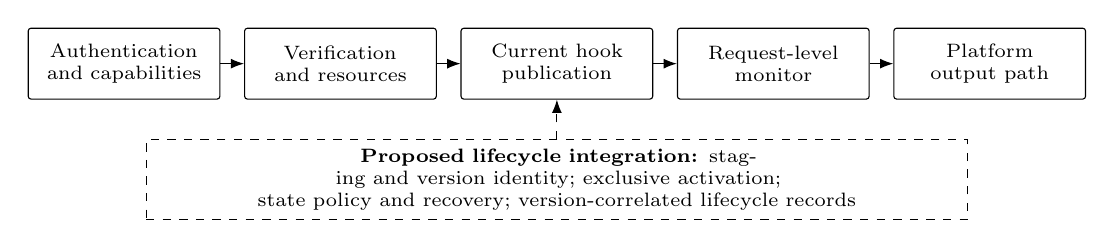
\begin{tikzpicture}[>=Latex,box/.style={draw,rounded corners=1pt,align=center,font=\scriptsize,minimum height=9mm,text width=22mm},node distance=3mm]
\node[box] (auth) {Authentication\\and capabilities};
\node[box,right=of auth] (verify) {Verification\\and resources};
\node[box,right=of verify] (pub) {Current hook\\publication};
\node[box,right=of pub] (monitor) {Request-level\\monitor};
\node[box,right=of monitor] (output) {Platform\\output path};
\draw[->] (auth)--(verify); \draw[->] (verify)--(pub); \draw[->] (pub)--(monitor); \draw[->] (monitor)--(output);
\node[draw,dashed,align=center,font=\scriptsize,text width=102mm,below=5mm of pub] (proposal) {\textbf{Proposed lifecycle integration:} staging and version identity; exclusive activation;\\state policy and recovery; version-correlated lifecycle records};
\draw[dashed,->] (proposal.north)--(pub.south);
\end{tikzpicture}
\caption{Existing component path (solid) and proposed lifecycle integration (dashed). Candidates enter from an external proposer. Current hook publication is not exclusive controller replacement. The figure does not claim independently validated physical-stop behavior.}
\label{fig:boundary}
\end{figure}

An existing bounded, overwrite-oldest RAM ring records request source, channel, authority, requested value, decision, reason, sequence, and timestamp. It is not a persistent lifecycle recorder or evidence that a physical output occurred. Likewise, generation-tagged handles and snapshot publication are useful primitives, but do not establish exclusive old-to-new controller activation. Coherent staging, state policy, recovery, and version-correlated lifecycle records remain \textbf{proposed}. End-to-end physical-stop independence remains unvalidated.

\begin{table}[t]
\centering
\caption{Measured cost per verifier invocation for synthetic straight-line programs. Intervals describe the time estimate reported by Criterion 0.5.1, not execution or installation latency.}
\label{tab:verifier}
\begin{tabular}{lr}
\toprule
Instructions & Reported 95\% confidence interval ($\mu$s)\\
\midrule
10 & 3.1151--3.1216\\
100 & 31.437--31.465\\
1,000 & 376.43--379.28\\
\bottomrule
\end{tabular}
\end{table}

Table~\ref{tab:verifier} reports retained measurements from a \textbf{single unpinned developer-host campaign on synthetic verifier workloads}: AMD Ryzen 7 7735HS, Linux x86\_64, Rust nightly 2026-07-02, and 100 Criterion samples per group after warm-up. These are reported 95\% intervals for Criterion's typical per-invocation time estimate. Raw console output and source/artifact hashes are retained; identifying provenance is withheld for review. The three rows are selected program sizes from its scaling workload. They are not independent deployment trials, a latency service-level objective, a cross-machine comparison, or measurements of agent-generated code. They show the cost of these verification cases only. No physical-actuation measurements, task improvements, or complete installation results are claimed.

\section{Evaluate adaptation and installation separately}
\label{sec:evaluation}
The evaluation unit should be a candidate \emph{within a versioned sequence}, not merely an isolated successful load. Record a timestamped lifecycle trace for each $u_i$: proposal, rejection or staging, activation if it occurs, observation, retention or recovery, and recovery completion or failure. Include the active artifact identity at each relevant event. Stage, activate, and recover are not mutually exclusive outcomes. Missing events and interrupted runs must remain visible.

\begin{table}[t]
\centering
\caption{Task quality and lifecycle correctness are separate axes. Correct installation does not imply that a task regression is detectable or recoverable.}
\label{tab:axes}
\small
\begin{tabularx}{\linewidth}{@{}lXX@{}}
\toprule
Task outcome & Lifecycle contract respected & Lifecycle contract violated\\
\midrule
Improvement & Intended result & Improvement masks an installation defect\\
Regression & Task regression despite correct installation & Compounded task and installation failure\\
\bottomrule
\end{tabularx}
\end{table}

\paragraph{Two hypothetical scenarios.}
In \textbf{motor-reflex adaptation}, an agent proposes bounded controller revisions after a payload or friction change. Include candidates that exceed requested authority or available resources, and inject activation failures, delayed old-version commands, and recovery requests. In \textbf{sensor-processing adaptation}, the agent revises a filter or classifier after distribution shift. Exercise incompatible state layouts, reset policies, exhausted staging budgets, and stale references. This second scenario tests whether the abstraction protects a changing processing pipeline as well as actuator access. Neither experiment has been performed in the case-study system.

\paragraph{Comparisons and independent labels.}
First replay the same ordered candidate artifacts and fault schedule against (i) frozen behavior, (ii) updates with the chosen action-assurance baseline, and (iii) that baseline plus lifecycle controls. Frozen behavior anchors task performance and availability; it is not an update-admission baseline. Match initial plant state, exogenous inputs or simulator seeds, and action-assurance configuration. This controlled replay tests installation effects; later plant states may diverge because installation decisions differ. Proposal generation is fixed.

A subsequent adaptive campaign should hold initial agents, task streams, and budgets fixed while permitting installation outcomes to affect later proposals; resulting proposal sequences may legitimately diverge. Unsafe ablations belong in simulation, not on unprotected hardware.

Label admissibility independently against explicit authority, validity, state, and resource contracts. Assign one terminal admission decision per candidate; account separately for pending decisions and timeouts. Report rejected inadmissible candidates divided by all labeled inadmissible candidates, accepted inadmissible candidates with the same denominator, and rejected admissible candidates divided by all labeled admissible candidates. A syntactically valid but unauthorized program is not a false rejection. Keep unresolved labels separate; rejection rate alone is not a safety score.

\paragraph{Measurements that distinguish the axes.}
Measure verification start-to-decision, activation request-to-first-authoritative invocation, and recovery request-to-declared-ready state, retaining failures and timeouts. Retain raw counts and report state-policy violations per activation, stale-command executions per executed command, and safety violations per unit of service time. Compare task performance before and after updates and against frozen behavior; preregister the loss threshold and observation window defining a catastrophic regression. Report these regressions per activated update and service-ready time per scheduled evaluation time. Report the fraction of activated updates that improve the task alongside false rejection and availability; use undefined, not zero, for empty denominators. Preserve candidate and version identities, requested and applied actions where observable, reason codes, uncertainty, and gaps. Repeat independent runs and summarize both per-run and pooled results without treating correlated control cycles as independent trials.

\section{Counterarguments, limitations, and research agenda}
\paragraph{A shield may be enough.}
This is a hypothesis to test. If the baseline already enforces version, state, authority, and resource transitions, a separate lifecycle component may be redundant. The relevant comparison is the contracts actually provided, not whether a system calls itself a shield or an updater.

\paragraph{The boundary may belong in middleware.}
A kernel is one design point, not the conclusion. Middleware with sufficiently restricted output access, explicit publication semantics, and a trusted downstream monitor may satisfy the same obligations. Compare assurance assumptions and measured costs, rather than attributing safety to implementation location.

\paragraph{Conservative admission can harm adaptation.}
Rejecting every proposal trivially avoids some update failures while preventing improvement. Useful evaluation must expose this tradeoff. Moreover, valid code can implement an unstable or ineffective controller; a correct installation lifecycle does not remove model uncertainty, guarantee detection of task regression, or make previous code safe in a changed environment. Recovery needs its own state, command-freshness, and re-arming conditions.

The present prototype establishes components and limited verification costs, not the proposed transaction or its benefits. The next evidence should be a matched, fault-injected update campaign measuring both axes, followed by closed-loop adaptation and attributable physical validation. The research question is whether explicit installation contracts add independently measurable protection at an acceptable cost. \textbf{For embodied agents, adaptation should not imply deployment.} Controlling how a proposal becomes authoritative is a systems problem that continual-learning evaluations should make visible.

\clearpage
\bibliographystyle{plainnat}
\bibliography{references}
\end{document}
